\documentclass[12pt]{article}

\usepackage{url}
\usepackage{color}
\usepackage{float}
\usepackage{array}
\usepackage{xcolor}
\usepackage{multirow}
\usepackage{graphicx}
\usepackage{booktabs}
\usepackage{colortbl}
\usepackage{hyperref}
\usepackage{spreadtab}
\usepackage{longtable}
\usepackage{pdflscape}
\usepackage[T1]{fontenc}
\usepackage[utf8]{inputenc}
\usepackage[english]{babel}
\usepackage[margin=1.5cm]{geometry}
\usepackage[format=hang,labelfont=bf,font=small]{caption}
\usepackage{mathtools, amsmath, amsthm, amssymb, amsfonts, mathpartir}

\begin{document}

\title{Homework 1: Deep Learning}
\author{Hugo Mantinhas 95592, João Silveira 95597}

\maketitle

\section*{Work Division}

\section*{Question 1}
\begin{itemize}
    \item \textbf{1. a)}
    \begin{figure}[h]
        \centering
        \begin{tabular}{|c|c|c|c|}
            \toprule
            & \textbf{Train} & \textbf{Validation} & \textbf{Test} \\
            \midrule
            \textbf{Perceptron} & 0.4654 & 0.4610 & 0.3422 \\
            \bottomrule
        \end{tabular}
        \label{tab:1a}
        \caption{Train and validation accuracies for the perceptron model}
    \end{figure}
    \begin{figure}[h]
        \centering
        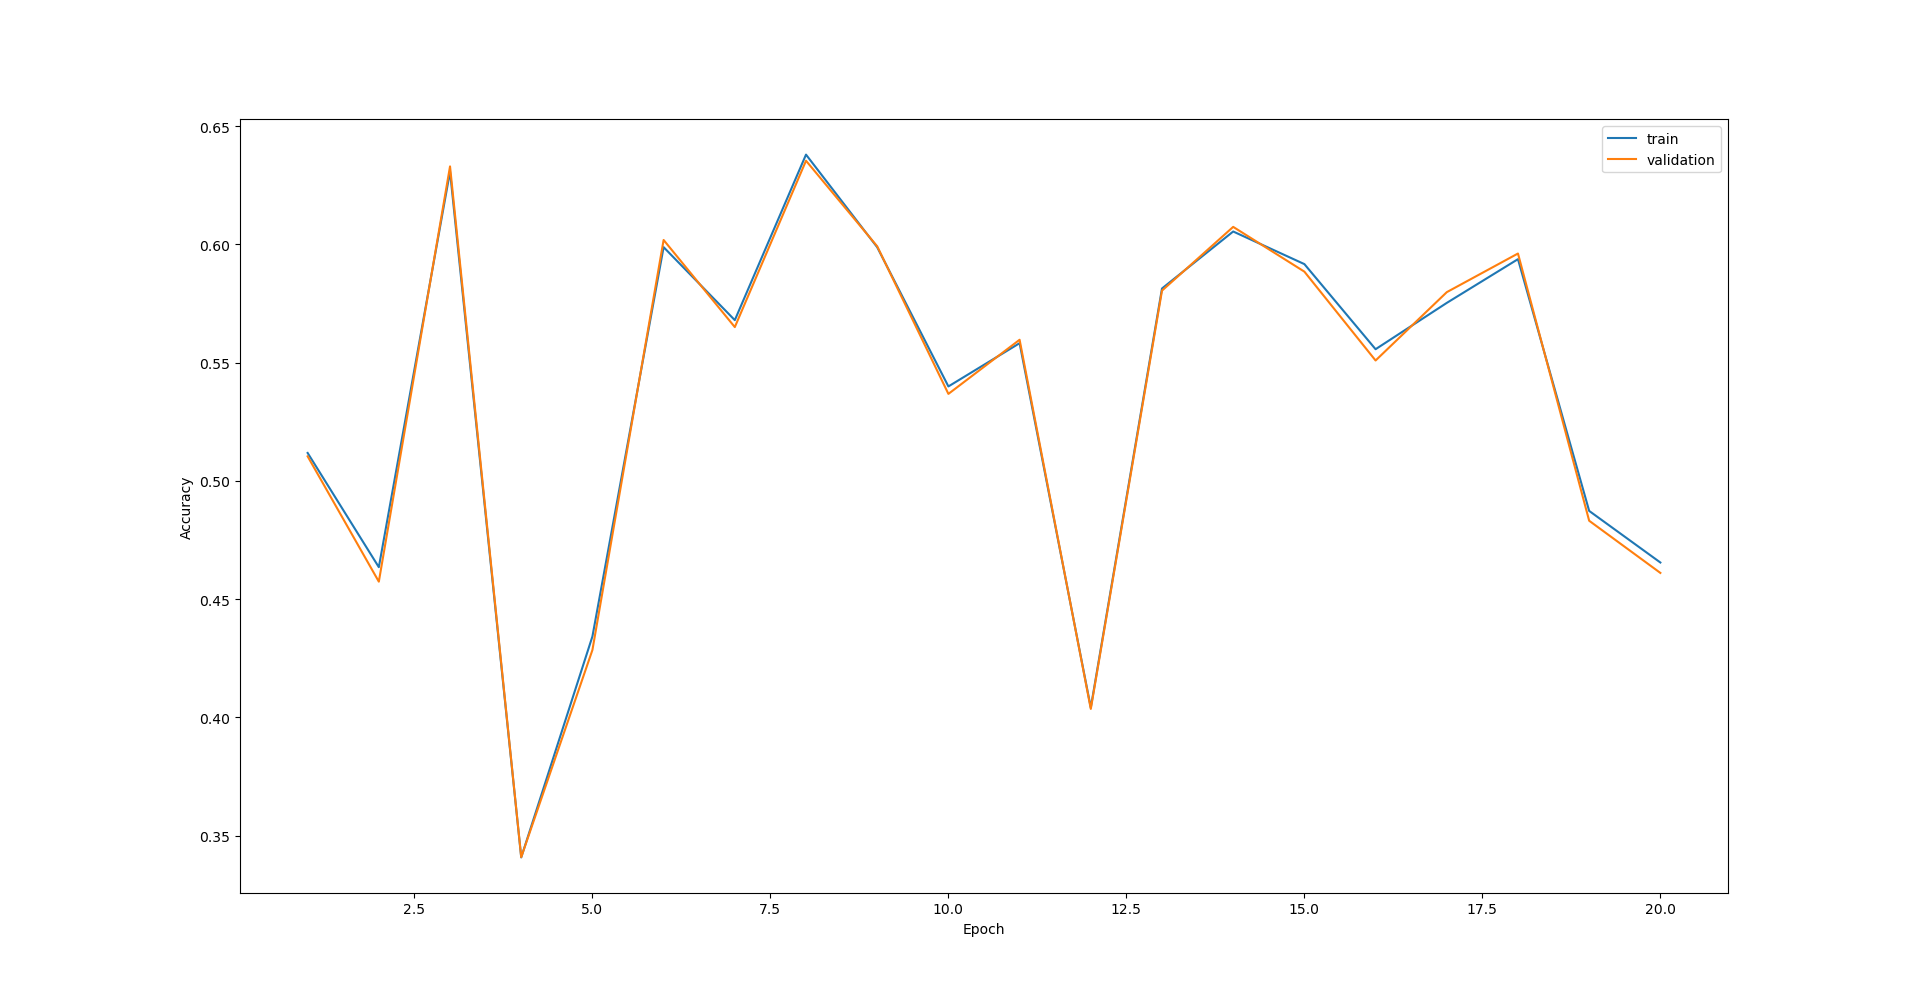
\includegraphics[width=0.45\textwidth]{../outputs/hw1-q1-1a.png}
        \caption{Train and validation accuracies for the perceptron model}
        \label{fig:1a}
    \end{figure}

    \item \textbf{1. b)} Analysing the plot with the learning rate of 0.01, we find that the weight update many times results in accuracy changes in the order of 5\%, in both directions. This suggests that the weight adjustments might be overshooting the optimal value. On the other hand, the learning rate of 0.001 results in a more stable learning process, with the accuracy changes being in the order of 1\% or less. Unlike the model trained with 0.01 learning rate, this one seems to be tending to grow over time. This suggests that the weight adjustments are closer to the optimal value. Although the accuracies don't look much different: 0.5784 for learning rate 0.01 and 0.5936 for learning rate 0.001; for the latter it shows a lot more stability in its accuracy across epochs.
    \begin{figure}[h]
        \centering
        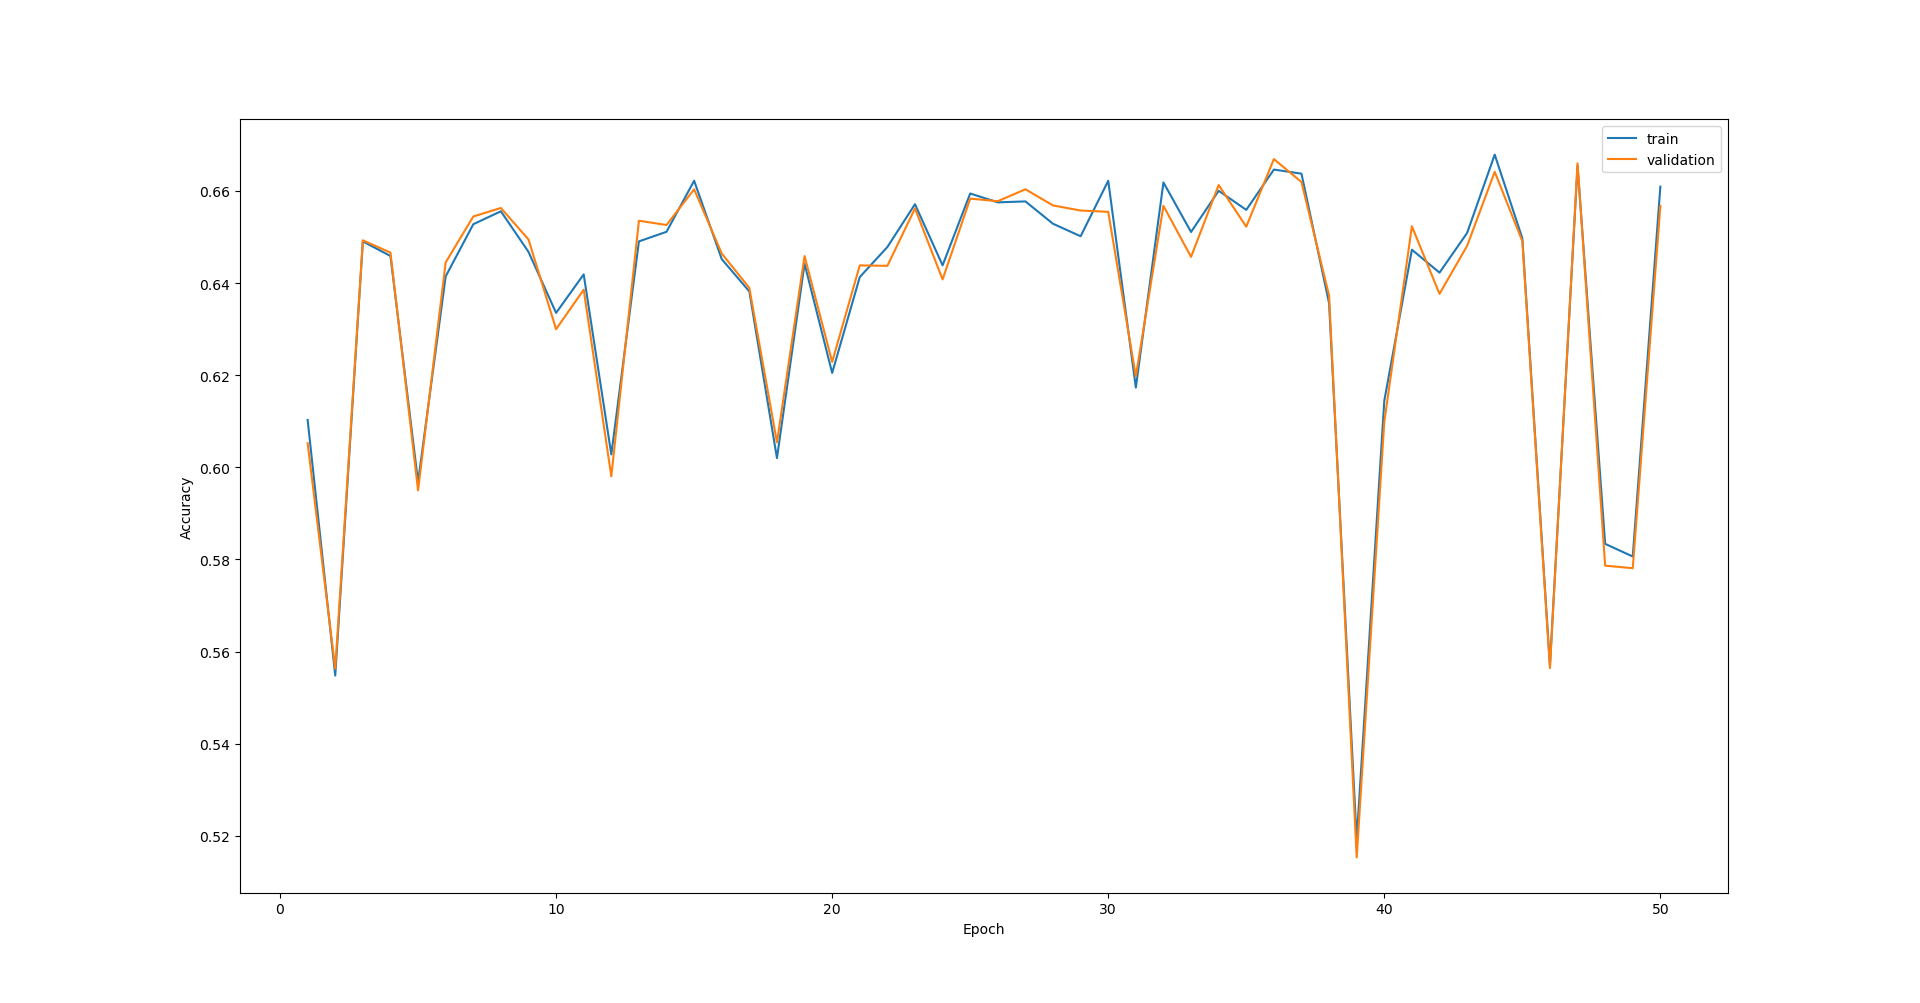
\includegraphics[width=0.45\textwidth]{../outputs/hw1-q1-1b.01.png}
        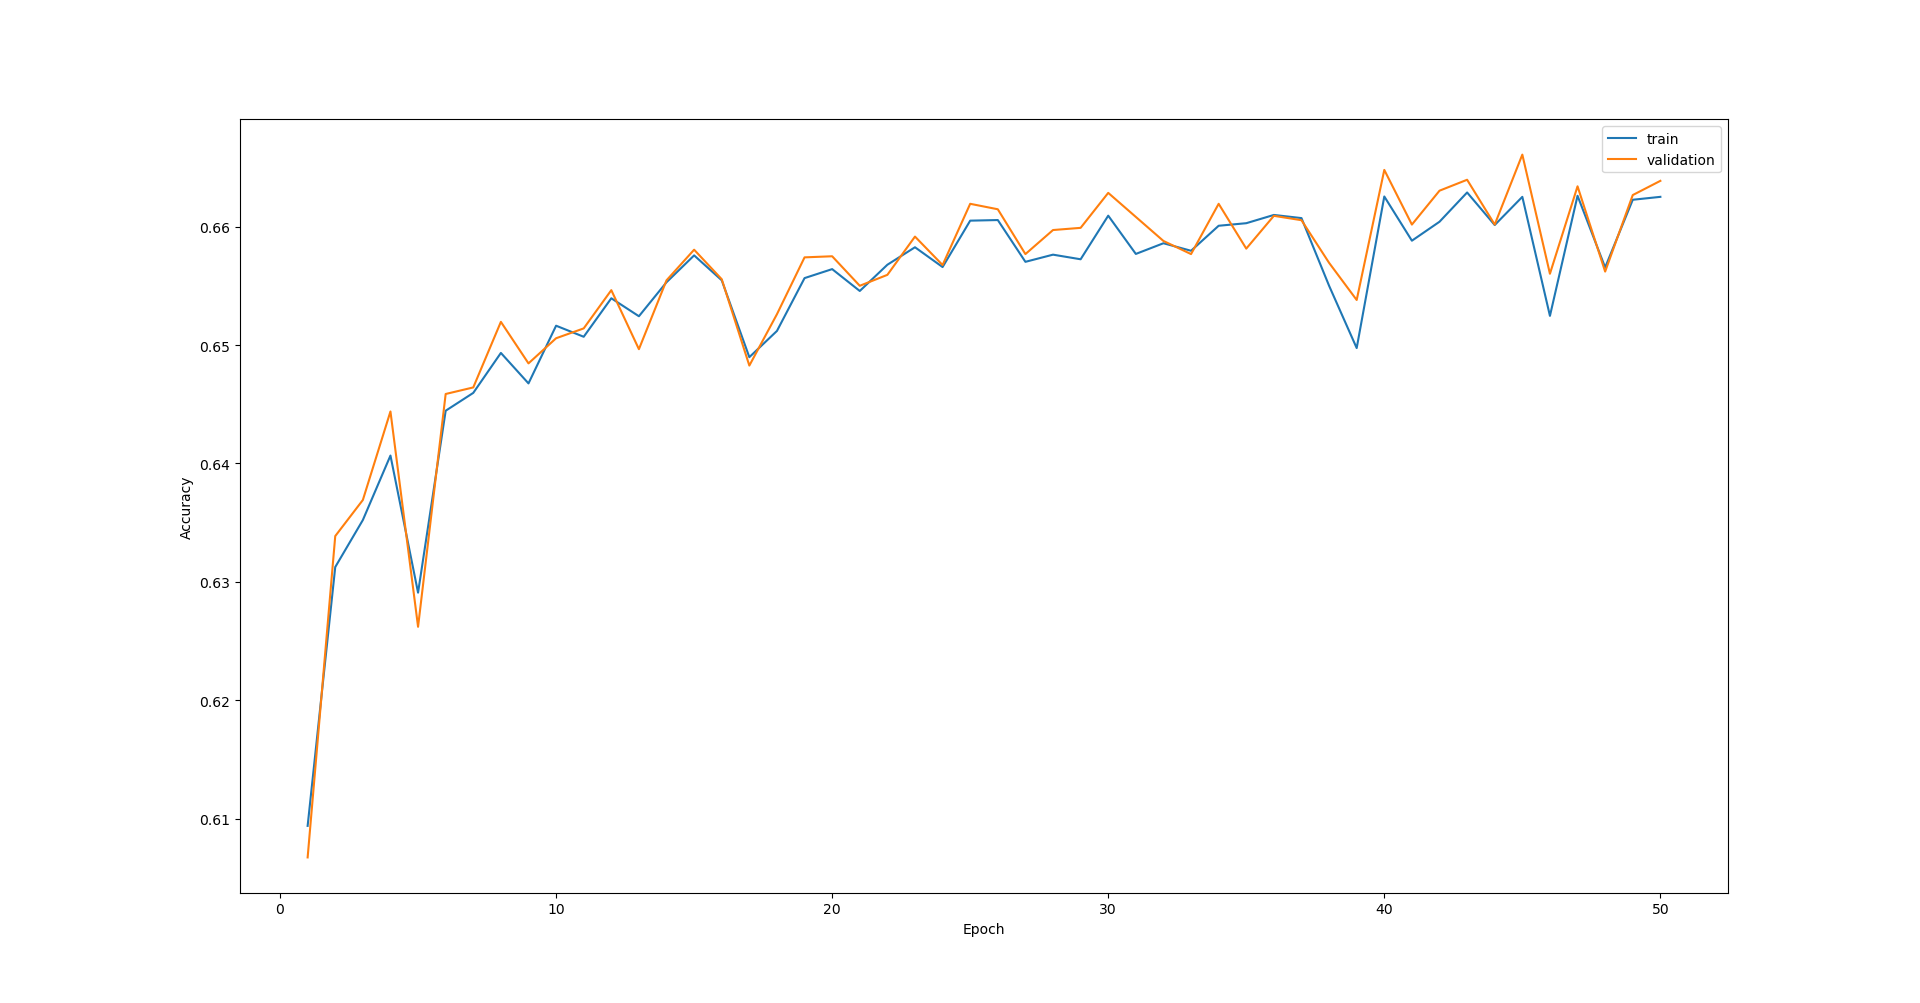
\includegraphics[width=0.45\textwidth]{../outputs/hw1-q1-1b.001.png}
        \caption{Train and validation accuracies for learning rates of 0.01 and 0.001}
        \label{fig:1b}
    \end{figure}
    \begin{figure}[h]
        \centering
        \begin{tabular}{|c|c|c|c|}
            \toprule
            & \textbf{Train} & \textbf{Validation} & \textbf{Test} \\
            \midrule
            \textbf{Learning rate 0.01} & 0.6609 & 0.6568 & 0.5784 \\
            \textbf{Learning rate 0.001} & 0.6625 & 0.6639 & 0.5936 \\
            \bottomrule
        \end{tabular}
        \label{tab:1b}
        \caption{Train and validation accuracies for learning rates of 0.01 and 0.001}
    \end{figure}
    \item \textbf{2. a)} This statement is true. A logistic regression model is a linear model, which means that it can only learn linearly separable data. On the other hand, a multi-layer perceptron using relu activations can learn to separate non-linearly separable data because of the non-linearity introduced by the relu activation function in between layers. However, it can be shown, by computing the Hessian matrix of the loss function, that the loss function of a logistic regression model using cross-entropy loss is always convex, while the loss function of a multi-layer perceptron, in general, is not. This means that the logistic regression model can be trained to a global optimum, while, with a multi-layer perceptron, we can never be sure that we have reached a global optimum.

    \item \textbf{2. b)} 
\end{itemize}

\section*{Question 2}

\end{document}